\section*{\centering Problematica}

Al acercarme a un comercio local ubicado en 
\textbf{Avenida San José de los Cedros 202, Cuajimalpa}, dirigido por la señora \textbf{Filomena Pera Vera}, 
pude percatarme de las dificultades que enfrentaba al momento de registrar sus ventas. Aunque actualmente se apoya en la herramienta 
\textbf{Microsoft Excel}, dicha solución resulta insuficiente para llevar un control preciso y eficiente de toda la mercancía disponible en su negocio.
\newline
\textbf{Imagen del negocio local}
\begin{center}
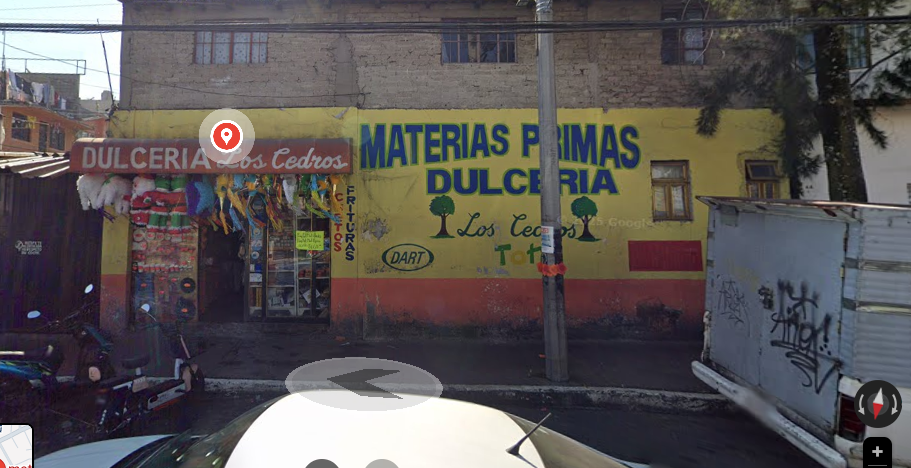
\includegraphics[width=0.5\textwidth]{imagenes/ubi.png}\par
\end{center}

\section*{Planteamiento de solución}
Durante una conversación con la señora Filomena, le expliqué algunas alternativas tecnológicas que podrían implementarse 
para optimizar la administración de su comercio, sin comprometer la seguridad ni la integridad de sus operaciones. 
Entre las posibles soluciones que le propuse, destacan las siguientes:

\begin{itemize}
    \item Reducir el exceso de mercancía que no tiene rotación, mediante análisis de inventarios para detectar productos con baja salida y tomar decisiones oportunas 
    (descuentos, promociones, devolución a proveedores, etc.).
    \item Identificar los productos estrella, es decir, aquellos con mayor demanda y rentabilidad, 
    para enfocar estrategias de venta y reposición prioritaria.
    \item Mejorar el sistema de puntos o lealtad del local, con el fin de incentivar las compras frecuentes y 
    premiar la fidelidad de los clientes.
    \item Gestionar de manera más eficiente las ventas a clientes recurrentes, incluyendo históricos de compras, preferencias y 
    condiciones especiales que permitan ofrecer un trato más personalizado.
    \item Tener un mejor control y registro de los recibos de ventas, facilitando el acceso rápido a la información para aclaraciones, 
    auditorías o análisis financieros.
\end{itemize}

Le comenté que la implementación de un sistema digital podría brindarle grandes beneficios, entre ellos: 
\begin{itemize}
    \item Automatización de procesos.
    \item Reportes en tiempo real.
    \item Una visión más clara de la salud financiera de su negocio.
\end{itemize}
 
Además, enfaticé que estas herramientas están disponibles y son muy accesibles (solo el uso de la computadora local y software de uso libre) y 
adaptadas a las necesidades de pequeños negocios, lo cual podría traducirse en mayor competitividad y crecimiento para su comercio.
